\documentclass{beamer}


\usepackage{listings}
\usepackage{soul}



\usepackage[
  binary-units=true,
  per-mode=symbol-or-fraction,
]{siunitx}


\usepackage[
  loop=true,
]{animate}

\definecolor{mygray}{rgb}{0.8,0.8,0.8}

%blues
\definecolor{comments}{RGB}{112,168,193}
\definecolor{stringcolor}{RGB}{43,114,144}
\definecolor{keywords}{RGB}{9, 72, 99}


\lstset{ %
  basicstyle=\fontsize{7pt}{7.4pt}\lstfont,        % the size of the fonts that are used for the code
  breakatwhitespace=true,          % sets if automatic breaks should only happen at whitespace
  breaklines=false,                % sets automatic line
  otherkeywords={repeated},        % if you want to add more keywords to the set
  commentstyle=\color{comments},   % comment style
  keepspaces=true,                 % keeps spaces in text, useful for keeping indentation of code (possibly needs columns=flexible)
  keywordstyle=\color{keywords},   % keyword style
  showspaces=false,                % show spaces everywhere adding particular underscores; it overrides 'showstringspaces'
  showstringspaces=false,          % underline spaces within strings only
  showtabs=false,                  % show tabs within strings adding particular underscores
  stepnumber=4,                    % the step between two line-numbers. If it's 1, each line will be numbered
  stringstyle=\color{stringcolor}, % string literal style
  tabsize=2,	                     % sets default tabsize to 2 spaces
}

\usetheme{m} % Use metropolis theme

%------------------------------------------------------------------------------
%------------------------------ Bibliographie ---------------------------------
%------------------------------------------------------------------------------

\usepackage[
  backend=biber,   % use modern biber backend
  firstinits=true,
  date=iso8601,
]{biblatex}
\addbibresource{references.bib}  % die Bibliographie einbinden
% \DefineBibliographyStrings{english}{andothers = {{et\,al\adddot}}}


\title{S-Bahn fahren mit dem Arduino.}
% \subtitle{Evaluating througput performance of the \stf on CTA Monte Carlo data}
\date{\today}
\author{Kai Brügge} \institute{TU Dortmund, Physik E5b, Astroteilchenphysik}
\begin{document}

\maketitle

\section{S-Bahn Fahren}

\begin{frame}[fragile]{S1}
  \begin{figure}[ht]
    \centering
      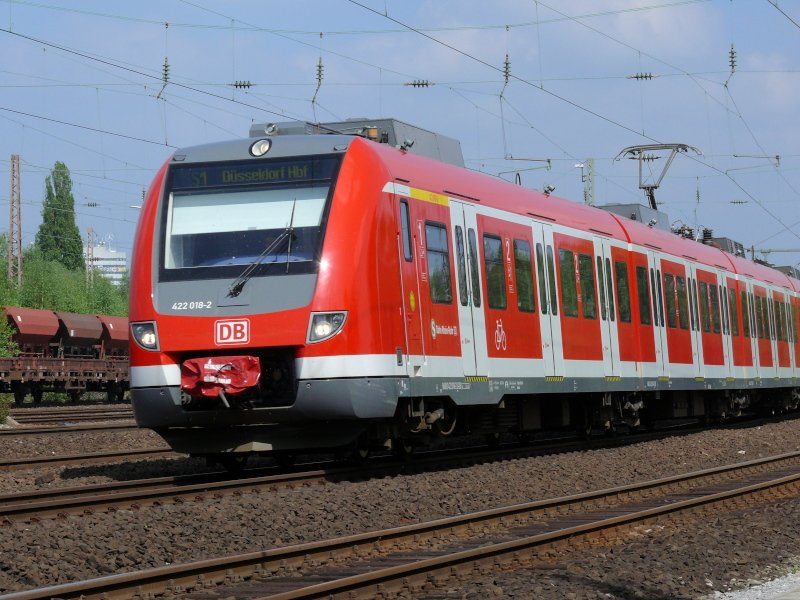
\includegraphics[width=0.6\textwidth]{pics/s1.jpg}
      \caption{Eine S-Bahn des Typs 422 in freier Wildbahn. }
      \label{fig:s1}
  \end{figure}
\end{frame}


\begin{frame}[fragile]{S1}
  Zitat Wikipedia zur den Zügen der S1:
  \begin{quote}
    Die DB-Baureihe 422/432 ist ein aus der Baureihe 423 weiterentwickelter vierteiliger elektrischer Triebzug für den Einsatz im Schienenpersonennahverkehr.
  \end{quote}
\end{frame}

\begin{frame}[fragile]{S1}
\begin{alertblock}{Die größte Frage der Menschheit: }
  Kommt die S1 pünktlich? \footnote{Eher nein.}
\end{alertblock}
\end{frame}


\begin{frame}[fragile]{Verkackte S1}

  Endlich gibt es die Antwort:

  \begin{figure}[ht]
    \centering
      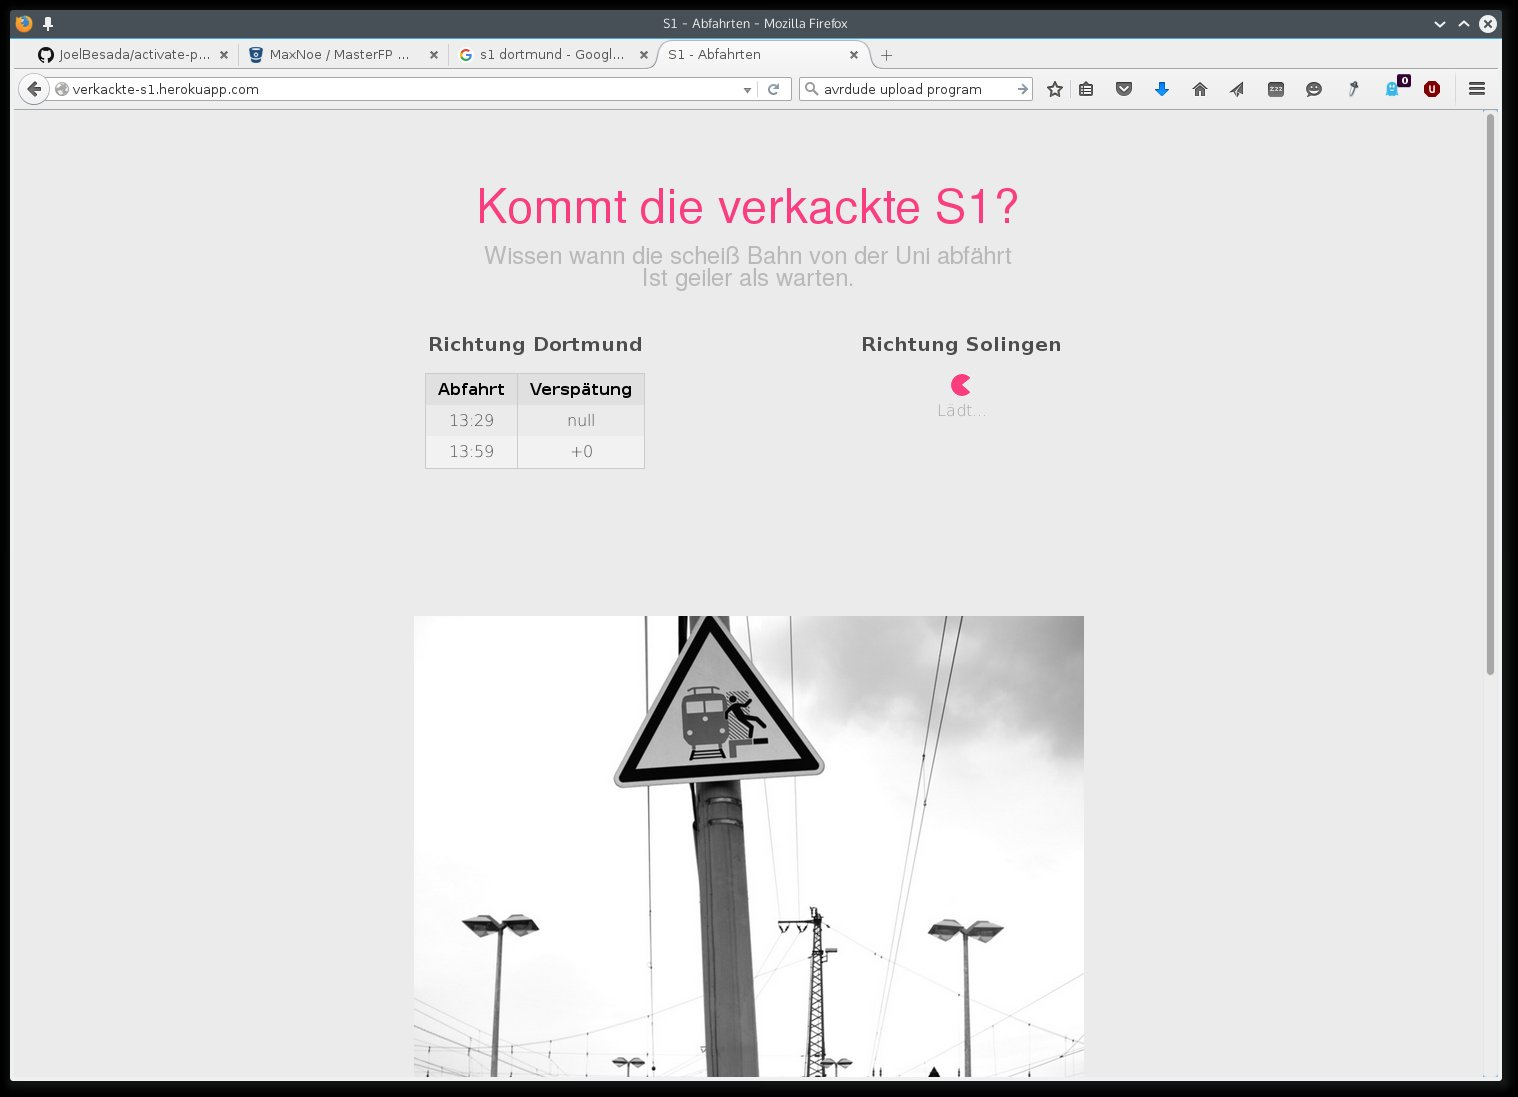
\includegraphics[width=0.7\textwidth]{pics/screen.jpg}
      \label{fig:screen}
  \end{figure}

\end{frame}

\section{Arduino}
\label{sec:Arduino}

\begin{frame}[fragile]{Mikrocontroller}
  Programmierung von Mikrocontrollern normalerweise extrem aufwendig.

  Bits in Registern müssen einzeln manipuliert werden.

  Nur primitive Datentypen. (keine Strings etc.)
\end{frame}

\begin{frame}[fragile]{Mikrocontroller}
  \begin{figure}[ht]
    \centering
      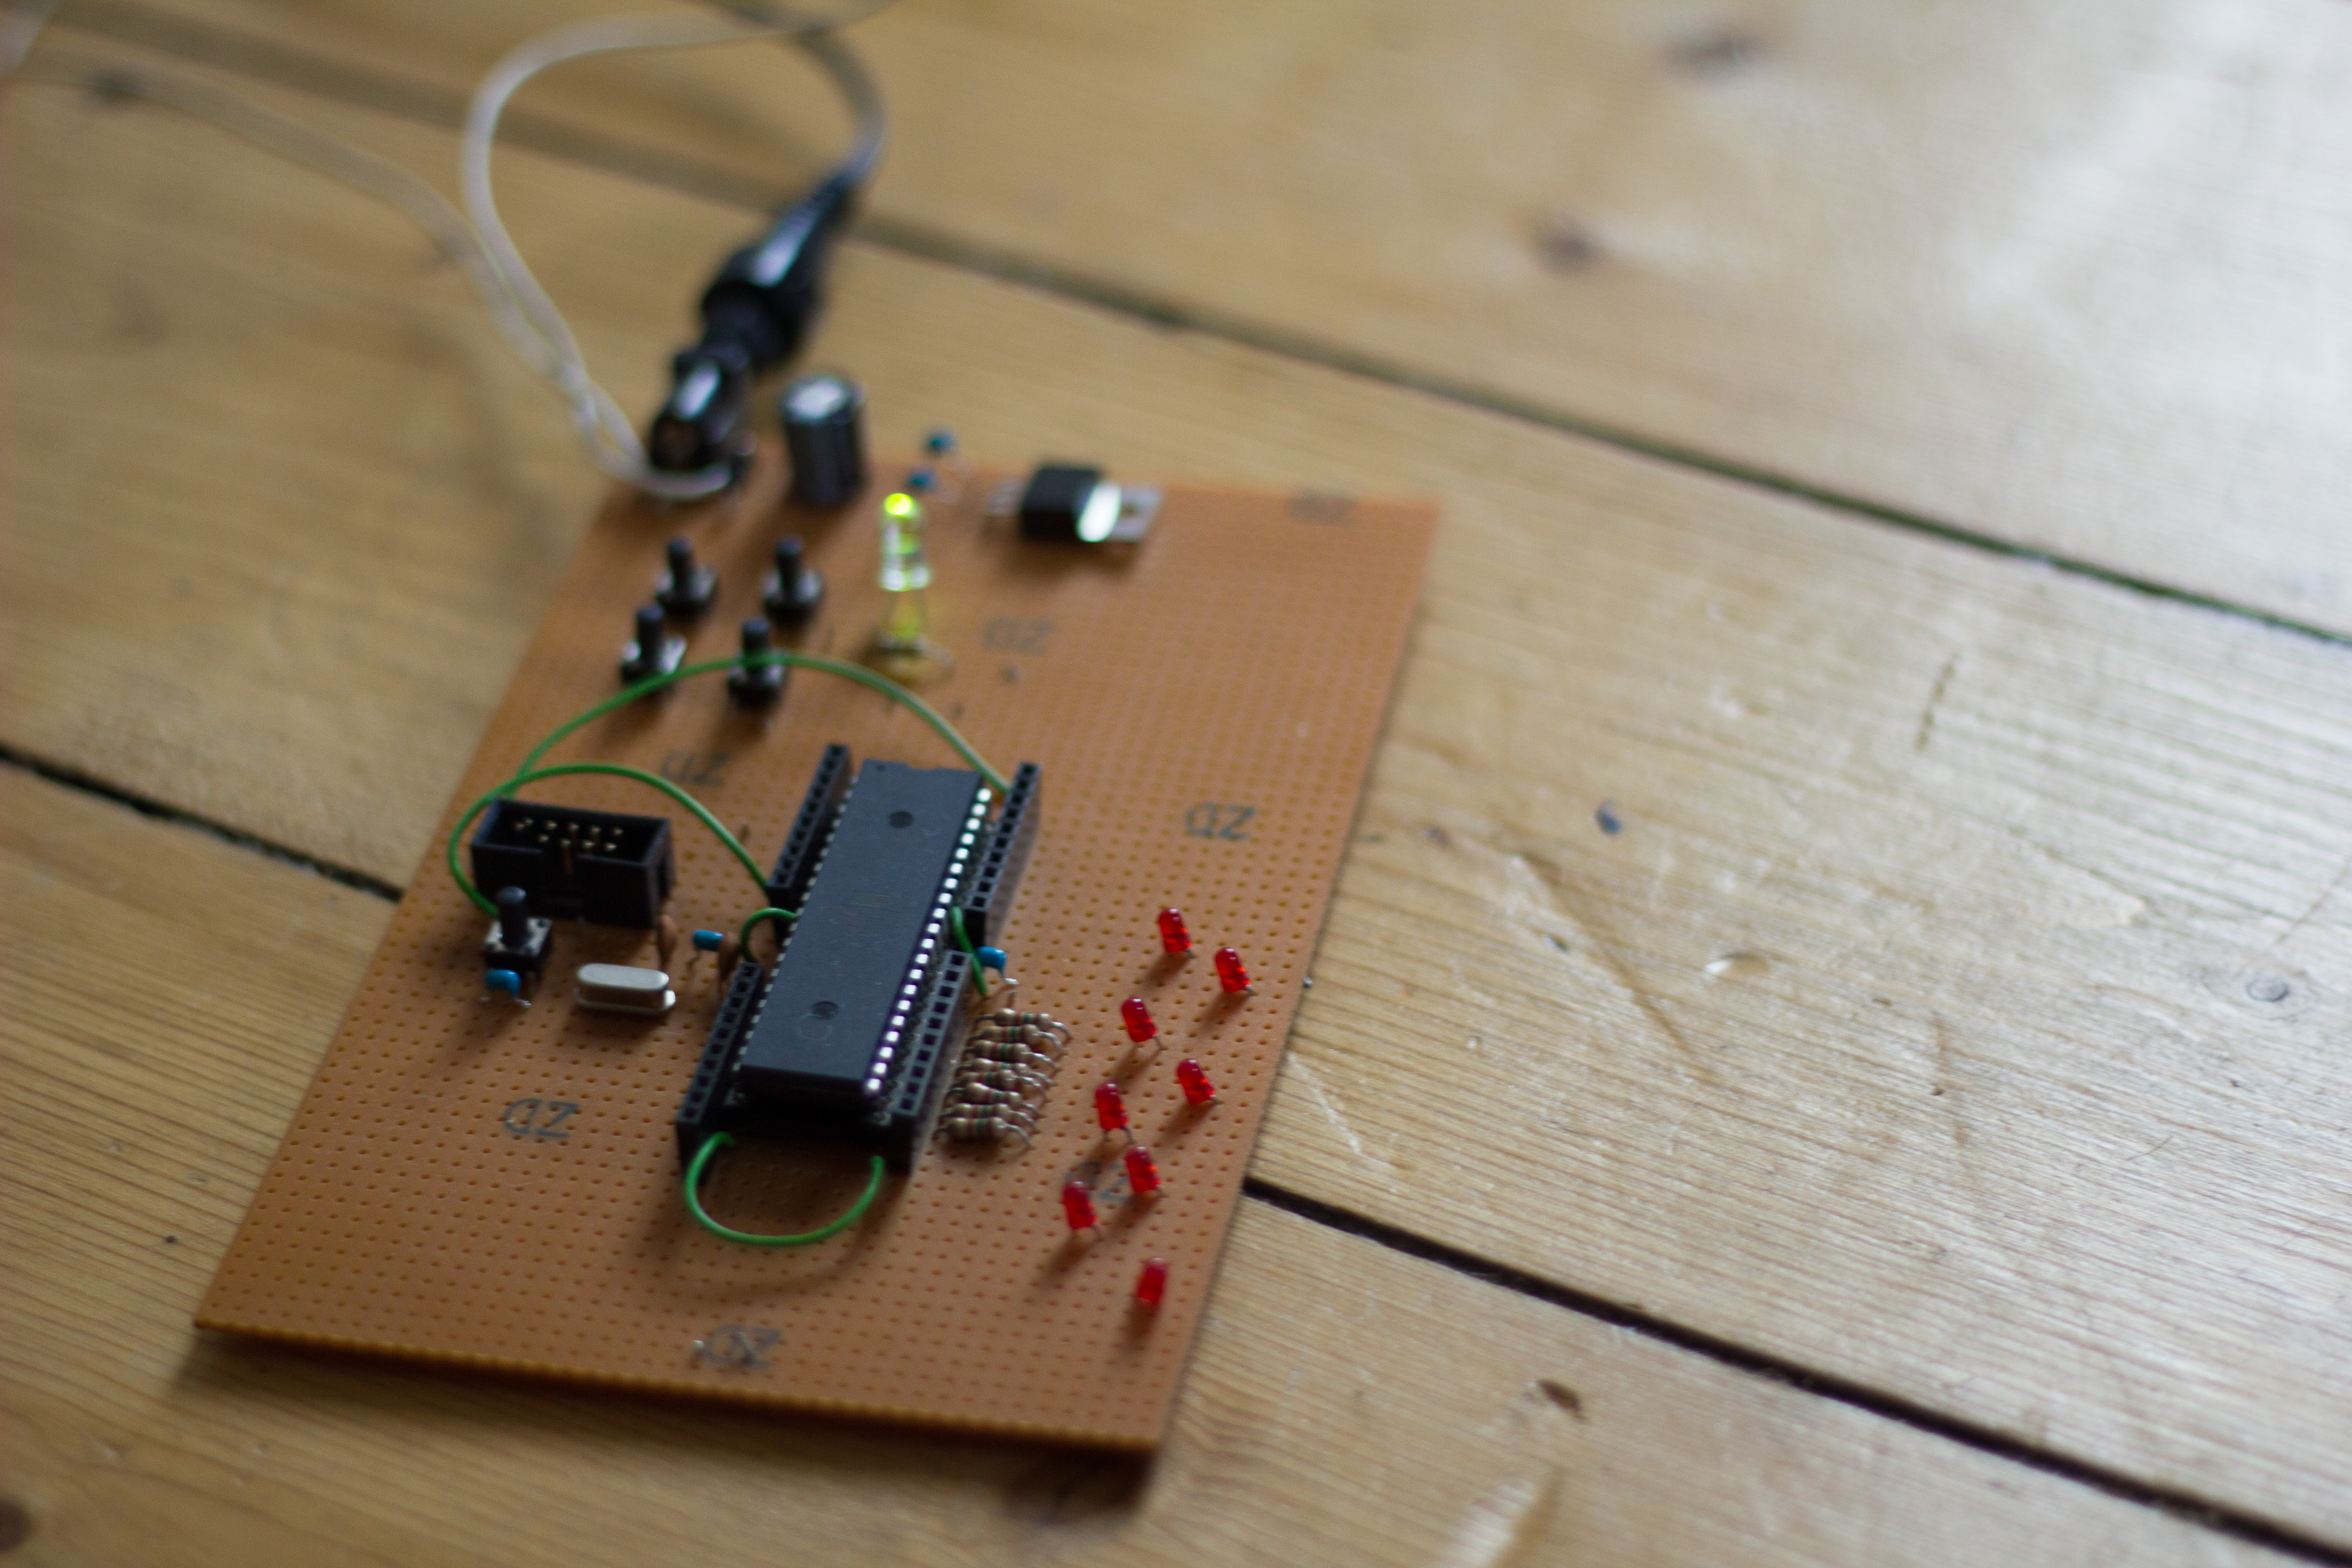
\includegraphics[width=0.85\textwidth]{pics/avr-1.jpg}
  \end{figure}
\end{frame}

\begin{frame}[fragile]{Arduino}
  \begin{alertblock}{Arduino}
    Sammlung von Hard- und Software komponenten für den leichten Einstieg.

    Große Anzahl an externen Bibliotheken für häufige Aufgaben und IO.
  \end{alertblock}
\end{frame}


\begin{frame}[fragile]{Arduino}
  Hier verwendet wurde der Arduino Ethernet.
  \begin{figure}[ht]
    \centering
      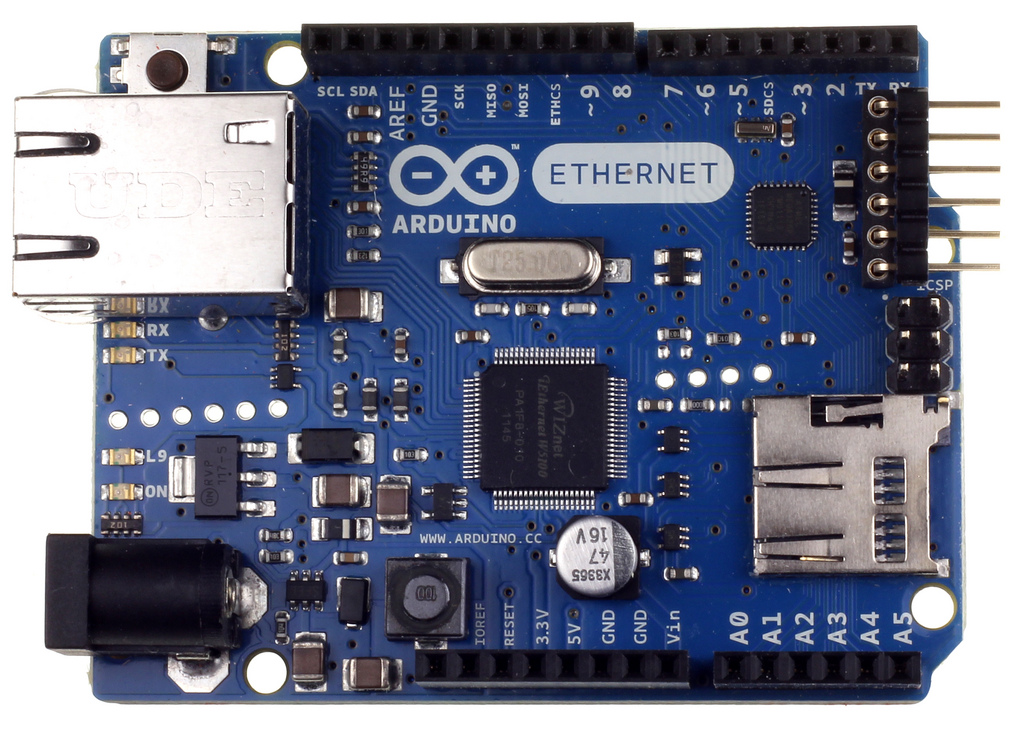
\includegraphics[width=0.75\textwidth]{pics/ArduinoEthernetFront.jpg}
  \end{figure}
\end{frame}


\begin{frame}[fragile]{Arduino}
  Kein USB Port vorhanden. Benötigt externen Programmer: AVR Dragon.
  \begin{figure}[ht]
    \centering
      \includegraphics[width=0.75\textwidth]{pics/avr-3.jpg}
  \end{figure}
\end{frame}

\begin{frame}[fragile]{Arduino}
  \begin{figure}[ht]
    \centering
      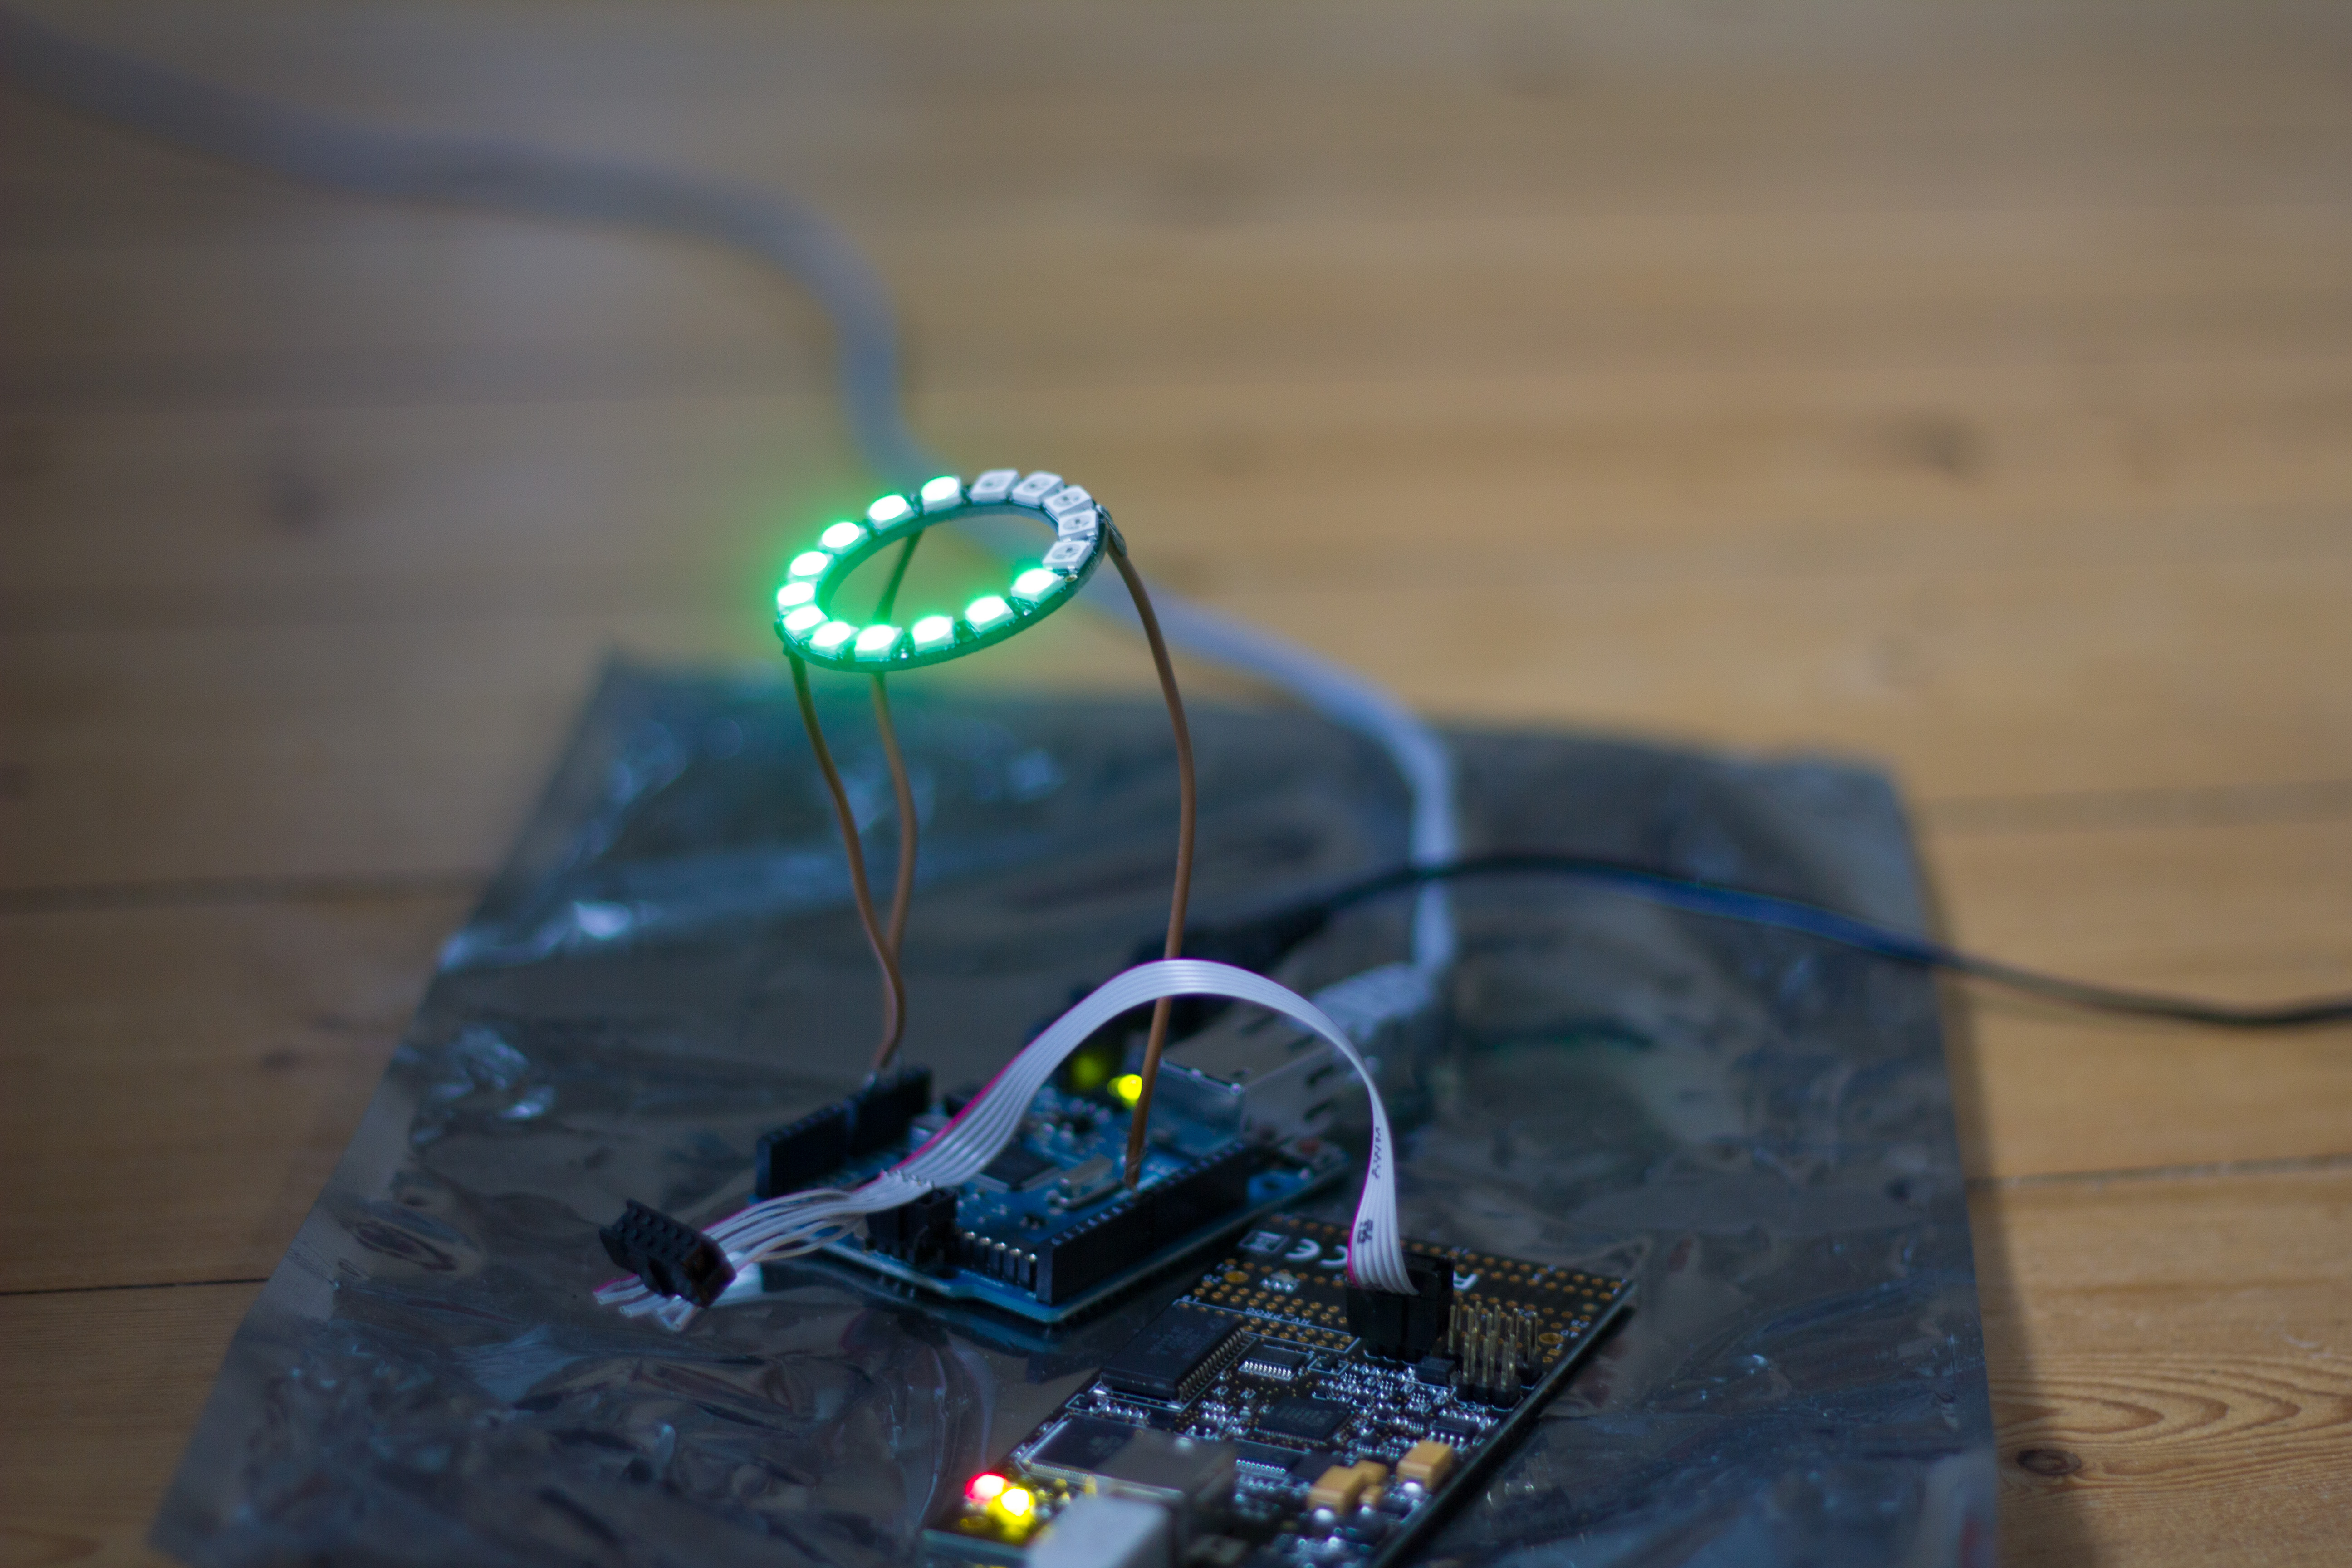
\includegraphics[width=0.85\textwidth]{pics/avr-2.jpg}
  \end{figure}
\end{frame}


\begin{frame}[fragile]{Platypus}
  \begin{figure}[h]
    \centering
      
\includegraphics[width=0.45\textwidth]{./platy.jpg}
  \end{figure}
\end{frame}


\end{document}
